\chapter{Dise\~no e Implementaci\'on del prototipo}

% **************************** Define Graphics Path **************************
\ifpdf
    \graphicspath{{Chapter4/Figs/Raster/}{Chapter4/Figs/PDF/}{Chapter4/Figs/}}
\else
    \graphicspath{{Chapter4/Figs/Vector/}{Chapter4/Figs/}}
\fi

Este cap\'itulo esta destinado a la comprensi\'on de los aspectos principales que hacen al dise\~no e implementaci\'on del prototipo para la nueva red aca\'emica. Cabe destacar, que en el mismo se toman como punto de partida las decisiones asumidas en el cap\'itulo anterior.

\section{Aspectos generales}

Como se menciona en el estado del arte, de acuerdo al enfoque SDN, en la arquitectura OpenFlow se tienen los planos de datos y control. En la arquitectura de OpenFlow, el plano de control es implementado por un software de control o comunmente llamado Controlador, y el plano de datos esta compuesto por los diferentes dispositivos de la red compatibles con OpenFlow.\\

La arquitetcura del prototipo, como puede apreciarse en la imagen ~\ref{fig:OpenSourceRArch0} se condice con esta estructura. Por un lado se tiene una red h\'ibrida IP/MPLS, donde cada nodo es uno de los routers opensource, cuya arquitectura se definir\'a m\'as adelante; y por otro se tiene a la entidad de control o Controlador sobre la cual se ejecuta la aplicaci\'on encargada de programar el comportamiento de cada uno de estos nodos. Finalmente, mediante el protocolo OpenFlow esta aplicaci\'on instala la configuraci\'on necesaria en cada nodo, para por ejemplo la implementaci\'on de un servicio de VPN particular.\\

\newpage
\begin{figure}[htbp!] 
\centering    
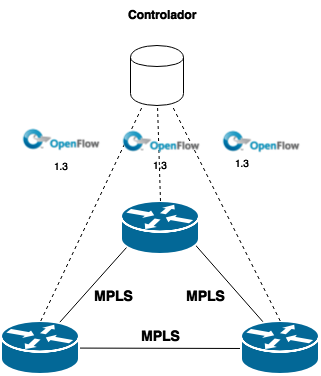
\includegraphics[width=0.4\textwidth]{Arch_Figure0}
\caption[OpenSourceRArch0]{Esquema general del prototipo}
\label{fig:OpenSourceRArch0}
\end{figure}

Se tienen entonces dos claras lineas de trabajo; el desarrollo del router opensource y el desarrollo de la entidad Controlador. 

\section{Router opensource}

Cada nodo del prototipo, es lo que en este trabajo se denomin\'o router opensource. Dicho router a su vez puede dividirse en diferentes componentes como se muestra en la figura~\ref{fig:OpenSourceRArch}.

\subsection{Plataforma de la PC}
El router esta constru\'ido sobre la plataforma de una PC de escritorio convencional. En particular se trabaja con un procesador Intel Core i7 de 64 bits, una Mother ASUS ROG Maximus Formula VI impuesta por los requerimientos de funcionamiento del hardware NetFPGA, 16GB de memoria DDR3, y un disco r\'igio de 1TB de capacidad. En el anexo [link] al anexo pueden encontrarse los detalles t\'ecnicos de la PC.

\subsection{Sistema Operativo}
Sobre el sistema operativo, se decidio trabajar con Ubuntu 12.04 sobre una arquitectura de 64 bits. Esta elecci\'on responde a dos criterios esencialmente. Por un lado la premisa de trabajar con sotware libre y de c\'odigo abierto preferentemente, nos llevo a buscar entre alternativas de sistemas operativos basado en GNU/Linux.

Por otro lado, el hardware NetFPGA asi como los proyectos existentes para su programaci\'on fueron desarrollados trabajando sobre la plataforma Fedora14. Teniendo presente esto, se intento infructuosamente instalar y configurar el hardware sobre dicha plataforma. Se probaron versiones m\'as recientes de esta plataforma como Fedora17 y Fedora19 obteniendo los mismos resultados. Entre las causas se detectaron incompatibilidades entre la Mother de la PC y algunas de las versiones del sistema operativo mencionado, falta de drivers apropiados para cable JTag con el que se programa el hardware, entre otros.

Finalmente tras probar con otras alternativas, se logro instalar y configurar exitosamente el hardware sobre la plataforma Ubuntu 12.04.\\

\subsection{Hardware NetFPGA}

El hardware NetFPGA funciona tanto conectado a una PC medianta un slot PCIe(modo servidor), como conectado \'unicamente a una fuente de energ\'ia el\'ectrica(modo standalone). En el dise\~no planteado, el hardware se encuentra conectado a la PC mediante un slot PCIe.

%\subsubsection{Instaaci\'on}
%La tarjeta NetFPGA se encuentra conectada a la PC mediante un slot PCIe. Para programarla, es necesario contar con la suite de Xilinx ISE instalada correctamente, con las respectivas licencias de productos, y un cable de programaci\'on JTAG. En particular, en el prototipo cada router cuenta con la suite de Xilinx ISE instalada, habilitando su reprogramaci\'on. Notar de todos modos que no es estrictamente necesario contar con la suite de Xilinx en el router para su funcionamiento.  

\subsubsection{Herramientas de Programaci\'on}

El hardware NetFPGA se programa utilizando un cable programador JTAG, y la herramienta Impact dentro de la suite de herramientas de Xilinx ISE. Para ello es indispensable contar con una estaci\'on de trabajo con dichas herramientas instaladas, habilitando la programaci\'on  del hardware NetFPGA que luego es colocado en la PC de cada router opensource. Cabe destacar adem\'as que la suite se compone por varias herramientas licenciadas para diferentes arquitecturas de chips; por ello es indispensable contar con el paquete de licencias apropiado al modelo de chip con que se trabaja (en nuestro caso Virtex5), y a las herramientas utilizadas. 

Esta estaci\'on de trabajo puede o bien ser la propia PC utilizada para el router opensource(alternativa utilizada en este proyecto), o bien puede ser una PC independiente a la utilizada para la construcci\'on de cada router.\\

%Cabe destacar que en la b\'usqueda de una plataforma compatible para la programaci\'on del hardware se probo con diferentes sistemas operativos como se menciono, logrando programarse el mismo en Windows XP y Ubuntu 12.04.

\subsubsection{Programaci\'on simple}
El hardware puede programarse de varias formas, una de ellas es lo que denominamos aqu\'i como programaci\'on simple. 

Esta estrategia consiste en la utilizaci\'on de la herramienta Impact y el cable JTAG para programar los chips FPGA y CPLD del hardware, con la implementaci\'on(bitfile) y arquitectura del proyecto con que se quiere programar la tarjeta.

Esta estrategia presenta como ventajas su simplicidad. No requiere de licencias pagas (puede descargarse una licencia gratuita para la herramienta Impact), y es el procedimiento descrito en la documentaci\'on de la plataforma NetFPGA.

Sin embargo presenta una desventaja importante; al producirse un ciclo completo de corriente (apagado y encendido del equipo), el hardware se desprograma. Concretamente el contenido del chip FPGA es borrado, y solo perdura el contenido del chip CPLD.\\

Tras constatarse este comportamiento, luego de revisar la documentaci\'on de la plataforma y recurrir al foro de la comunidad NetFPGA, se accedio a una lista de correos mediante la cual se establecio una comunicaci\'on con el equipo de desarrollo de NetFPGA[poner link al apendice de problemas tecnicos]. Este di\'alogo adem\'as de ayudarnos a comprender mejor el funcionamiento de la plataforma, desemboco en la segunda estrategia de programaci\'on.

\subsubsection{Programaci\'on persistente}
El hardware NetFPGA cuenta en su arquitectura con dos unidades de memoria flash(Flash A y Flash B). En la programaci\'on persistente estas unidades se utilizan para almacenar la programaci\'on del hardware, permitiendo que en cada encendido el chip FPGA se programe a partir del contenido de una de estas unidades. Por defecto el chip siempre se programa con el contenido de la memoria Flash A, habilitando su reprogramaci\'on desde la memoria Flash B v\'ia el bus PCIe.\\

Para que un proyecto se pueda persistir en una de las memorias Flash, y luego reprogramar el chip FPGA a partir de dicha memoria, debe presentar cierta arquitectura especial. En particular el proyecto ReferenceNIC, asi como tambi\'en ReferenceSwitch y Reference Router tienen esta caracter\'istica.

En el procedimiento empleado, inicialmente se programa el hardware con el proyecto ReferenceNIC utilizando la Programaci\'on Simple. Luego es necesario transformar la implementaci\'on del proyecto(archivo bitfile) en un archivo con el formato requerido para la memoria flash(archivo binario). Esto \'ultimo se realiza utilizando herramientas que incluye la plataforma de NetFPGA. Finalmente utilizando la herramienta \textbf{pcieprog} de la plataforma, se transfiere el archivo generado a una de las memorias flash.\\

Cabe destacar que durante la ejecuci\'on de este procedimiento se detectaron algunos errores y comportamientos inesperados en el hardware. Esto fue reportado al equipo de desarrollo de NetFPGA a traves de una lista de correos, reportandose en total 2 bugs que fueron solucionados y contemplados en la siguiente actualizaci\'on del repositorio de c\'odigo fuente. Por m\'as detalles acerca de estos bugs y su resoluci\'on referirse al siguiente ap\'endice[link al apendice].\\

Por otro lado, esta estrat\'egia de programaci\'on utiliza herramientas de la suite de Xilinx que requieren de licencias pagas. Este detalle se constato experimentalmente en la ejecuci\'on del proyecto. Cabe destacar que la informaci\'on de error proporcionada por la herramienta al intentar ejecutarla sin las licencias correspondientes, asi como la documentaci\'on disponible no suguieren de forma intuitiva un problema de licencias. Por ello, teniendo la intuici\'on de que se trataba efectivamente de un problema de licenciamiento se solicitaron licencias adicionales a trav\'es del programa de apoyo universitario de Xilinx.

Tras pasar varias semanas a la espera de una respuesta, se establecio un contacto con docentes del IIE de Facultad de Ingenieria. Desde el IIE se contesto que no trabajaban con esta plataforma pero que lo hab\'ian hecho en un pasado; facilit\'andonos un conjunto de licencias con el que se logro resolver el problema de licenciamiento. 

Mucho tiempo despu\'es el programa universitario de Xilinix don\'o un paquete de licencias entre las cuales se encontraban las necesarias. Por m\'as detalles acerca de este problema referirse al siguiente ap\'endice [link al apendice y problema tecnico].

%%%%%%%%%%%%%%%%%%%%%%%%%%%%%%%%%%
%Cabe destacar que este procedimiento no funciona correctamente. El proyecto PCIPrograming presenta alg\'un tipo de BUG(al momento de grabar una memoria se queda en loop), y tras reportar este comportamiento en la comunidad de NetFPGA se nos suguiere utilizar el proyecto ReferenceNIC que presenta el diseno de la arquitectura similar al PCIPrograming. Siguiendo esta sugerencia se logra programar correctamente el hardware de forma persistente, constatandose que al realizar un ciclo de corriente completo el hardware no se desprograma. Por esta raz\'on la estrategia de programaci\'on utilizada en el hardware es la programaci\'on persistente aqu\'i detallada.\\

%Vale la pena destacar tambi\'en, que al programarse el hardware desde cualquiera de las unidades de memoria Flash, en particular con el proyecto Reference NIC el hardware no se comportaba de la forma esperada. Tras constatarse que esto no sucedia con versiones anteriores del c\'odigo fuente del proyecto, nuevamente se le reporta lo sucedido al soporte de NetFPGA obteniendo como respuesta una sugereencia para emparchar el c\'odigo, y la promesa de que ser\'ia solucionado en la siguiente versi\'on (lo cual pudimos constatar).

%Tras estas modificaciones se logra obtener el hardware programado de forma persistente. De todos modos luego de ejecutarse una serie de pruebas se constatan comportamientos an\'omalos en capa f\'isica de las interfaces de la placa (podemos meter la descripcion). Nuevamente se reporta el comportamiento a la comunidad de NetFPGA desde donde se nos suguiere un parche para el driver, aparentemente causante del error. Se realizan los cambios y todo anda yuju!  

%\subsubsection{Programaci\'on vol\'atil y persistente}
%El hardware puede programarse en forma vol\'atil(la programaci\'on se pierde al cortarse la corriente), y en forma persistente mediante una unidad flash de memoria.

%La primera alternativa tiene la ventaja que implica un procedimiento simple, no requiere de licencias de software pagas puesto que se realiza utilizando la herramienta Impact(viene en la suite de Xilinx ISE) para la cual se pueden obtener una licencia gratuita, y a su vez es el procedimiento empleado en la documnetaci\'on disponible del hardware NetFPGA. Por estas razones, esta estrat\'egia es la utilizada inicialmente para la programaci\'on del hardware NetFPGA en el router.

%No obstante un nodo del prototipo de red para la RAU, no puede desprogramarse ante un posible corte de corriente, quedando in\'util e incapaz de recuperarse en forma independiente. Debe ser capaz de recuperarse de forma aut\'onoma, al menos en lo que concierne a la programaci\'on del hardware NetFPGA.\\

%La segunda alternativa por otro lado no presenta este inconveniente, y por ello es la estrat\'egia utilizada finalmente para la programaci\'on del hardware. No obstante como se menciona anteriormente dicha estrat\'egia no figura claramente dentro de la documentaci\'on de la plataforma NetFPGA. Es por ello que tras iniciar una comunicaci\'on con el equipo de desarrollo de dicha plataforma, y utilizando diferentes herramientas como un foro de la comunidad de NetFPGA y una lista de correos, se logra dar con esta estrat\'egia de progrmaci\'on, gracias a la pronta respuesta de el equipo de NetFPGA.

%Existen dos formas de programar el hardware NetFPGA: una vol\'atil en memoria y otra persistente mediante una unidad flash de memoria. La primera alternativa fue utilizada en el inicio de este proyecto en principio por ignorancia, detectandose en cierto punto que tras realizar un ciclo de apagado y encendido del equipo la tarjeta se desprogramaba. No obstante esta modalidad tiene la ventaja que no requiere de licencias especiales para programar la placa; solo se requiere la herramienta Impact(disponible mediante una licencia gratuita) y el bitfile precompilado del proyecto con el cual se vaya a programar el hardware.

%Por otro lado, programar el hardware de forma persistente tiene la ventaja de que no debe ser reprogramado cada vez que el equipo es apagado y prendido nuevamente(proceso que requiere de abrir la PC, conectar el cable programador JTAG y cargar los m\'odulos con un tiempo aproximado no menor a 10 minutos). Este comportamiento se condice m\'as con el esperado por el router opensource; es entendible que un nodo del prototipo se quede sin corriente y se apague momentaneamente. Luego el mismo debe ser capaz de recuperarse correctamente sin la intervenci\'on de un programador.

%En el prototipo, cada nodo es programado utilizando el m\'etodo persistente. Esto implica primero cambiar la modalidad de programaci\'on del hardware a PCIe, lo cual se hace cambiando de posici\'on tres switches en la placa. Luego, para programar en particular el hardware con el proyecto Reference NIC, se programa de forma vol\'atil el mismo con dicho proyecto. Una vez finalizada la programaci\'on se generan un archivo binario a partir del bitfile del proyecto Reference NIC, con el cual luego utilizando la utilidad \textbf{pciprog} que viene con la suite de proyectos y herramientas de NetFPGA se almacena la programaci\'on de la tarjeta en una de las dos memorias flash con las que cuenta el hardware(en el prototipo siempre se utiliza la memoria A). De esta forma el hardware en cada ciclo de interrupci\'on de corriente, se programa desde la memoria flash.\\

%[Aca hay que reformular lo de arriba para decir, hubieron 2 bugs. Uno que impedia programar el hardware con el proyecto pci programing y que terminamos usando el reference nic (quedaba en loop cuando se queria escribir en las memorias). Luego que se pudo proramar pero cuando levantaba desde las flash no andaba como tarjeta pero si en programacion normal. Esto llevo a hablar con netfpga, parche correciones a archivos, solucionado. Se incorpora en nueva version.]

[que paso con las licencias]

%%%%%%%%%%%%%%%%%%
%Por otro lado en cuanto al hardware NetFPGA, como se menciona anteriormente el mismo se encuentra programado para comportarse como una tarjeta de red convencional, mediante el proyecto ReferenceNIC. Inicialmente se tuvieron inconvenientes para lograr persistir la programaci\'on de dicha placa. En un principio por falta de experiencia la programaci\'on del chip FPGA se estaba realizando en forma vol\'atil. Luego se aprendi\'o la forma correcta para programar dicho hardware en forma persistente pero el comportamiento era el mismo. Esto se debi\'o a una serie de BUGs en el proyecto Reference NIC que tras ser reportados en la lista de correos del equipo de soporte de NetFPGA, se nos comunico una parche para solucionar dicho problema. Tras esta intervenci\'on la persistencia en la programaci\'on del hardware se logro exitosamente.\\

%Tambi\'en se tuvieron problemas con la suite de desarrollo y programaci\'on Xilinx ISE con la que se programa el hardware. En particular este software asi como otras herramientas del SDK de Xilinx son licenciadas. Algunas de estas licencias no solo son costosas si no que distinguen a su vez entre las herramientas de la suite sobre las que se tiene derechos y el hardware utilizado. En particular para la arquitectura del chip FPGA utilizado por la placa NetFPGA(Virtex5), las licencias gratuitas o de prueba no contemplan las herramientas de compilaci\'on. Entonces si bien la programaci\'on vol\'atil del hardware con el proyecto Reference NIC es posible pura y exclusivamente utilizando licencias gratuitas, dado que este proyecto viene precompilado, la programaci\'on persistente del hardware con el mismo proyecto no lo es. Esto se debe a que se debe compilar otro proyecto (NOMBRARLPO) y generar archivos especiales que posteriormente se guardan en unidades flash de memoria de la NetFPGA; y estas acciones requieren de licencias pagas. 

%Finalmente tras solicitar estas licencias atrav\'es del plan de apoyo a universidades de la empresa Xilinx, se obtuvieron X-licencias entre las cuales se consiguieron las licencias requeridas. Por m\'as detalles acerca del procedimiento de programaci\'on del hardware referirse al anexo [link al anexo] secci\'on [numero de secci\'on]. 
 
\subsection{Open vSwitch}

En el router, el plano de datos de OpenFlow es implementado totalmente por Open vSwitch; por ello tambi\'em se encuentra condicionado a las funcionalidades de Open vSwitch. En relaci\'on a estos aspectos, durante el desarrollo del prototipo se relevo lo siguiente:

\begin{enumerate}
\item Parte de las funcionalidades de Open vSwitch, se encuentran disponibles en modo kernel, y otra parte en modo usuario. Estas \'ultimas presentan un nivel de performance muy pobre en comparaci\'on a la primera; y en particular las funcionalidades de MPLS se encuentran solamente disponibles en modo usuario.

\item De acuerdo a las notas de liberaci\'on de la \'ultima versi\'on oficial de Open vSwitch(2.3.1), 
se garantiza el soporte a MPLS en las operaciones de match, push y pop, para una \'unica etiqueta, as\'i como el posterior procesamiento del paquete de acuerdo al pipe de OpenFlow. A su vez dichas operaciones son soportadas solamente en modo usuario.

\item Experimentalmente se comprobo que si bien las operaciones de match y Push funcionaban correctaente para Open vSwitch v2.3.1, la operaci\'on de Pop no funcionaba correctamente. Este comportamiento se encontraba reportado como bug, y fue solucionado en la versi\'on de desarrollo de Open vSwitch. A su vez junto con esta mejora se incorporo el soporte para las operaciones de match, push y pop en hasta 3 etiquetas MPLS en modo usuario, lo cual fue comprobado experimentalmente en este trabajo.

\item Problema con interfaces con IP

\end{enumerate}

%Por otro lado en relaci\'on a las componentes de software, el router se compone de un sistema operativo escritorio basado en linux, con las instalaciones de Open vSwitch, Quagga y el agente de gesti\'on SNMP. Nuevamente por mayores detalles acerca de las versiones de software utilizadas, sistema operativo entre otros detalles refierase al anexo [link al anexo].\\

\newpage
\begin{figure}[htbp!] 
\centering    
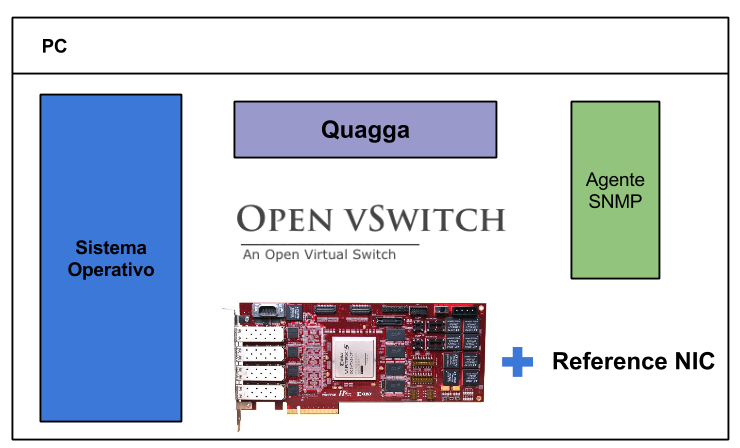
\includegraphics[width=0.7\textwidth]{Arch_Figure1}
\caption[OpenSourceRArch]{Diagrama de componentes del router open source}
\label{fig:OpenSourceRArch}
\end{figure}

\subsection{Quagga}

\subsection{Agente SNMP}

Se explicaron las principales caracter\'isticas del dise\~no e implementaci\'on del router, ahora es el turno del Controlador.

\section{Entidad Controlador}
Con respecto al Controlador, vale la pena destacar solamente las componentes de software dado que en relaci\'on al hardware, el mismo esta basado en una PC de escritorio. En la imagen ~\ref{fig:OpenSourceRArch3} se aprecian los componentes que constituyen al Controlador.\\

Al igual que el router, el Controlador consta de un sistema operativo sobre el cual posteriormente se instalan las diferentes componentes de software utilizadas. Particularmente esta compuesto por la suite de ruteo Quagga, un modulo encargado de la sincronizaci\'on de la informaci\'on topl\'ogica, un gerente SNMP, y finalmente el software de control SDN Ryu, sobre el cual se ejecuta la aplicaci\'on RauFlow.

\begin{figure}[htbp!] 
\centering    
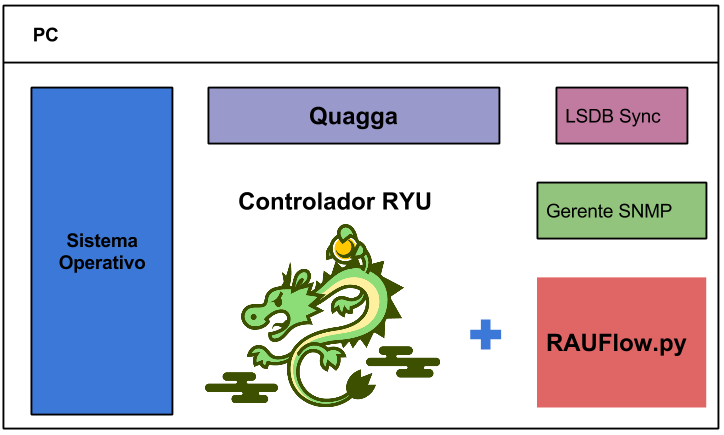
\includegraphics[width=0.6\textwidth]{Arch_Figure3}
\caption[OpenSourceRArch3]{Diagrama de componentes del Controlador}
\label{fig:OpenSourceRArch3}
\end{figure}

\section{Dise\~no general}

De esta forma, el prototipo para la nueva versi\'on de la red acad\'emica, se compone principalmente de algunos nodos construidos en base al router opensource, y un dispositivo controlador. Como se puede observar en la imagen \ref{fig:OpenSourceRArch4} los nodos se comunican con el Controlador mediante el protocolo OpenFlow como se explico con anterioridad, habilitando de esta forma a que el plano de datos sea programado por el plano de control. Por otro lado las diferentes instancias de Quagga distribu\'idas en cada nodo de la red y en el dispositivo controlador, se comunican mediante un canal IP con el objetivo de aprender la topolog\'ia y diseminar la informaci\'on de ruteo. Finalmente el gerente SNMP interactua con los diferentes agentes SNMP localizados en cada nodo mediante el canal IP, para obtener infirmaci\'on adicional acerca de cada nodo. 

\begin{figure}[htbp!] 
\centering    
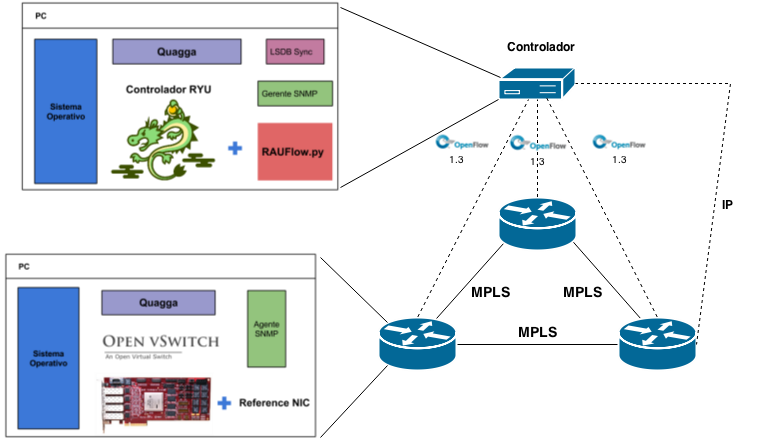
\includegraphics[width=0.9\textwidth]{Arch_Figure4}
\caption[OpenSourceRArch4]{Vista l\'ogica del prototipo}
\label{fig:OpenSourceRArch4}
\end{figure}